The figures in this section illustrate the Simulink model used to simulate A Downwind turbine with feed forward optimum pitch control. This is the feed forward controller analyzed in Chapter \ref{Chapter3}. Figure \ref{figB-7} shows the top level Simulink system. Much of the figure looks similar to Figure \ref{figB-1}, which illustrates the baseline (or upwind) turbine. In fact, the FAST block and all of the components of the baseline closed loop controller are present in Figure \ref{figB-7}. However, there is a new component. In the lower left corner there is a Feed Forward Controller subsystem that sends a FF Pitch Command signal to the Pitch Controller subsystem.
 
\begin{figure}[ht]
	\centering
		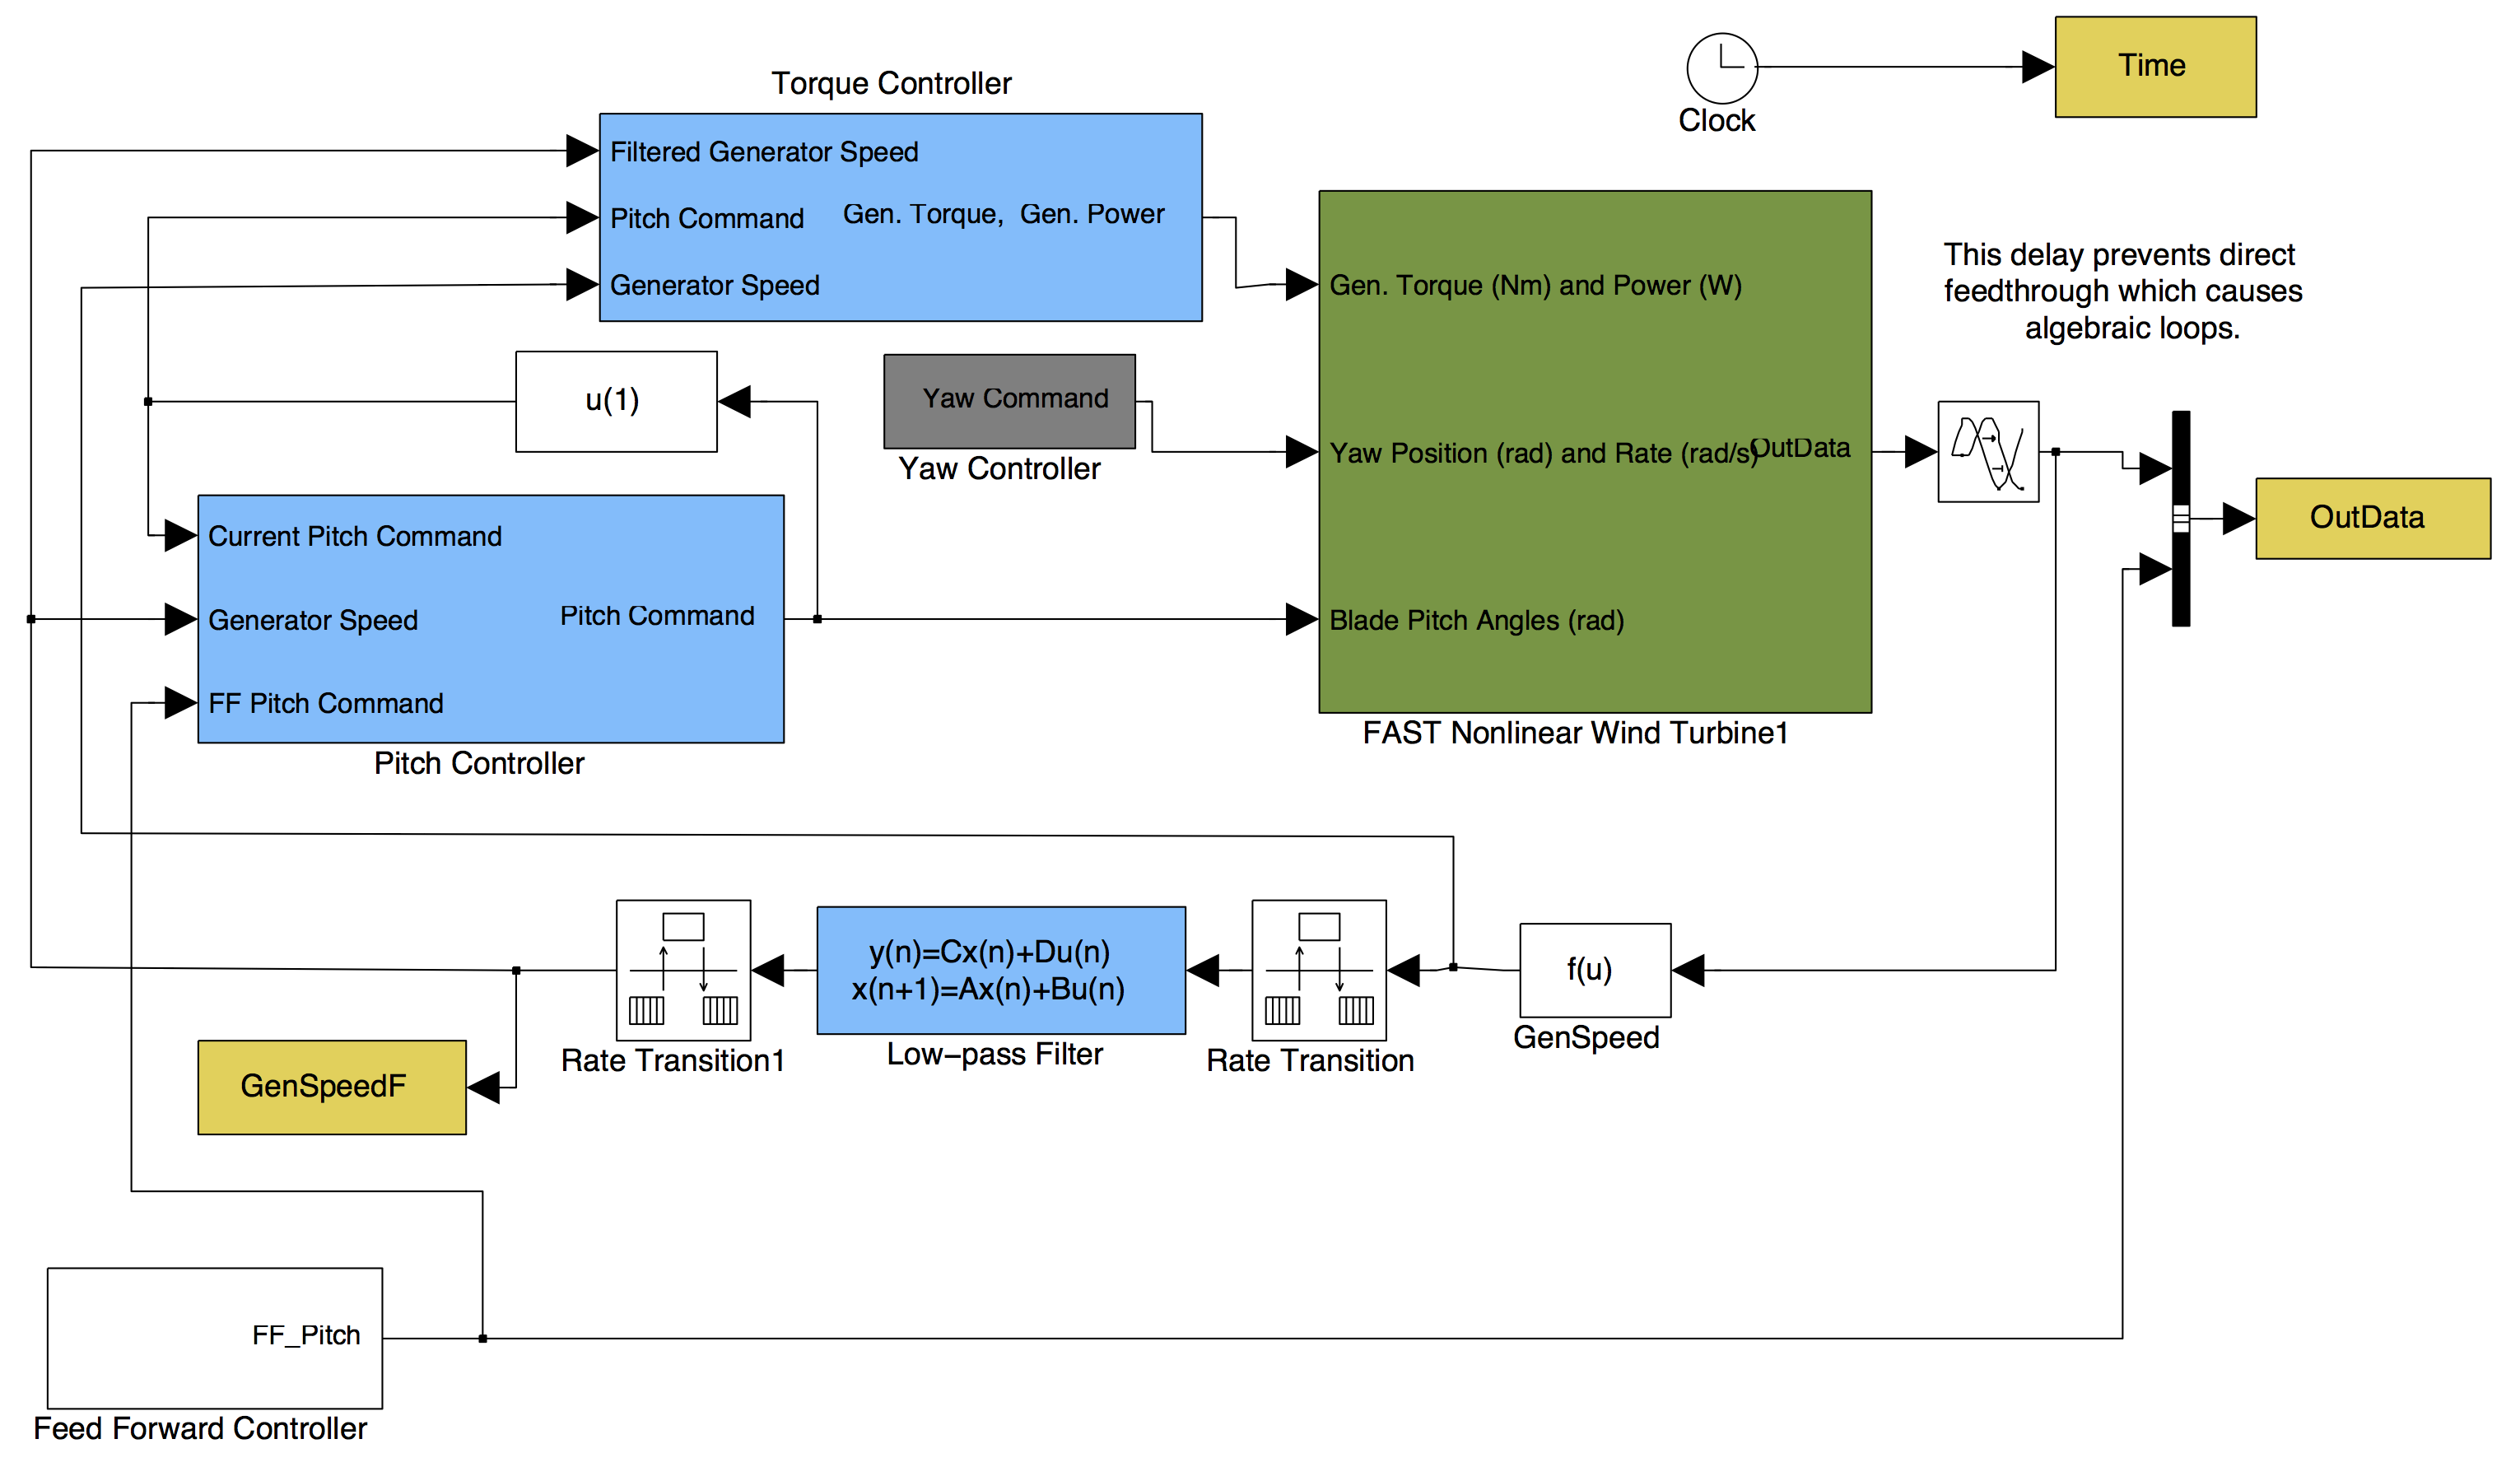
\includegraphics[width=\linewidth]{Figures/AppendixBFigures/FF_Pitch1.png}
	\caption{Top level Simulink system for model of NREL 5-MW with feed forward optimal pitch control.}
	\label{figB-7}
\end{figure}

Figure \ref{figB-8} shows the Feed Forward Controller subsystem. This subsystem is simple because most of the calculations are done prior to the simulation by a set of Matlab files. The FF Dynamic Wind Speed Lookup block contains a time history of the dynamic feed forward velocity ($U_{ff}$), which has been generated based on the output data from the Upwind Turbine simulation. Dynamic feed forward velocity is described in Section \ref{section3-3-3} and Equation \ref{eq3-3}. To save space, the Matlab files that are used to process Upwind Turbine output data and create the FF Dynamic Wind Speed Lookup table have not been included in this appendix. Those Matlab files are fairly long and several sets of files were required for the different sets of assumptions and operating conditions used in Chapter \ref{Capter3}. The FF Pitch Lookup Table contains a table relating dynamic feed forward velocity to the corresponding optimum pitch angle that will keep the turbine at a 12.1 RPM rotor speed. The relationship between dynamic feed forward velocity and optimum pitch angle is shown in Figure \ref{fig3-11}.

\begin{figure}[ht]
	\centering
		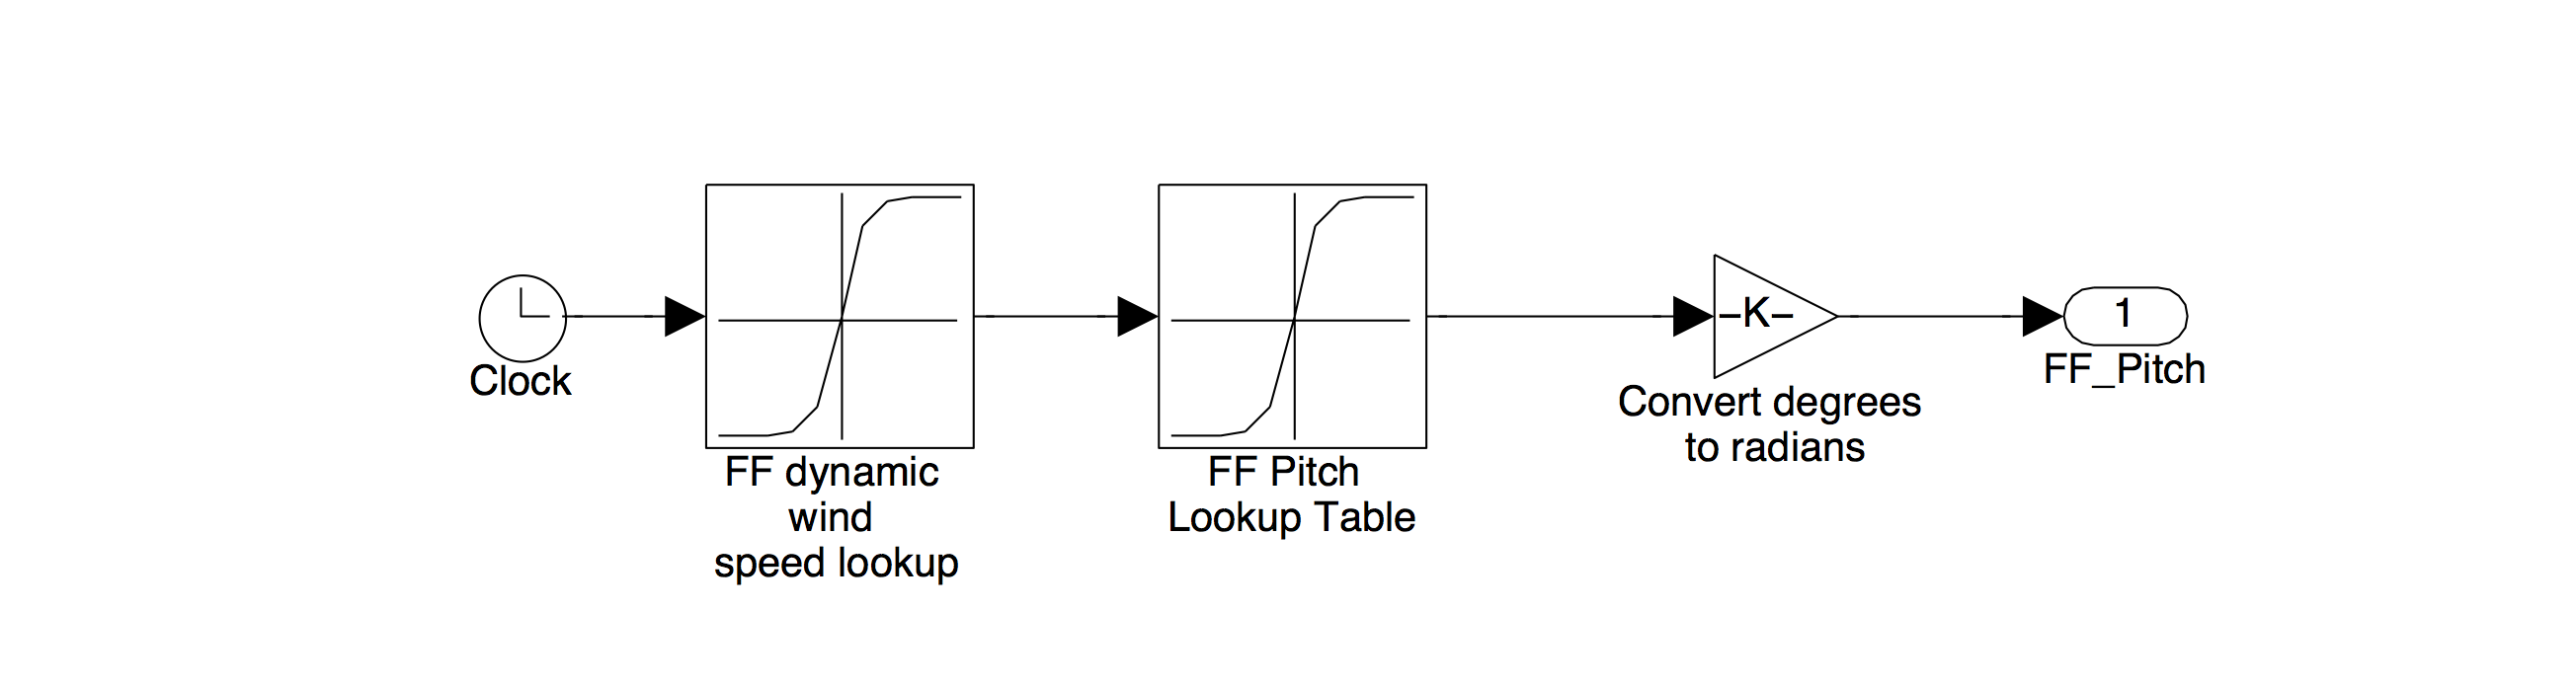
\includegraphics[width=\linewidth]{Figures/AppendixBFigures/FF_Pitch2.png}
	\caption{Feed Forward Controller subsystem for Simulink model of NREL 5-MW with feed forward optimal pitch control.}
	\label{figB-8}
\end{figure}

The Pitch Controller subsystem is shown in Figure \ref{figB-9}. It has been modified to accept the FF Pitch Command. The entire closed loop pitch control system is still present in this subsystem. The feed forward pitch is added to the Blade Pitch Command coming from the Total Pitch Command subsystem. This combined pitch command, from the closed loop controller and the feed forward controller, is then fed through the blade pitch actuator model before being passed to FAST.

\begin{figure}[ht]
	\centering
		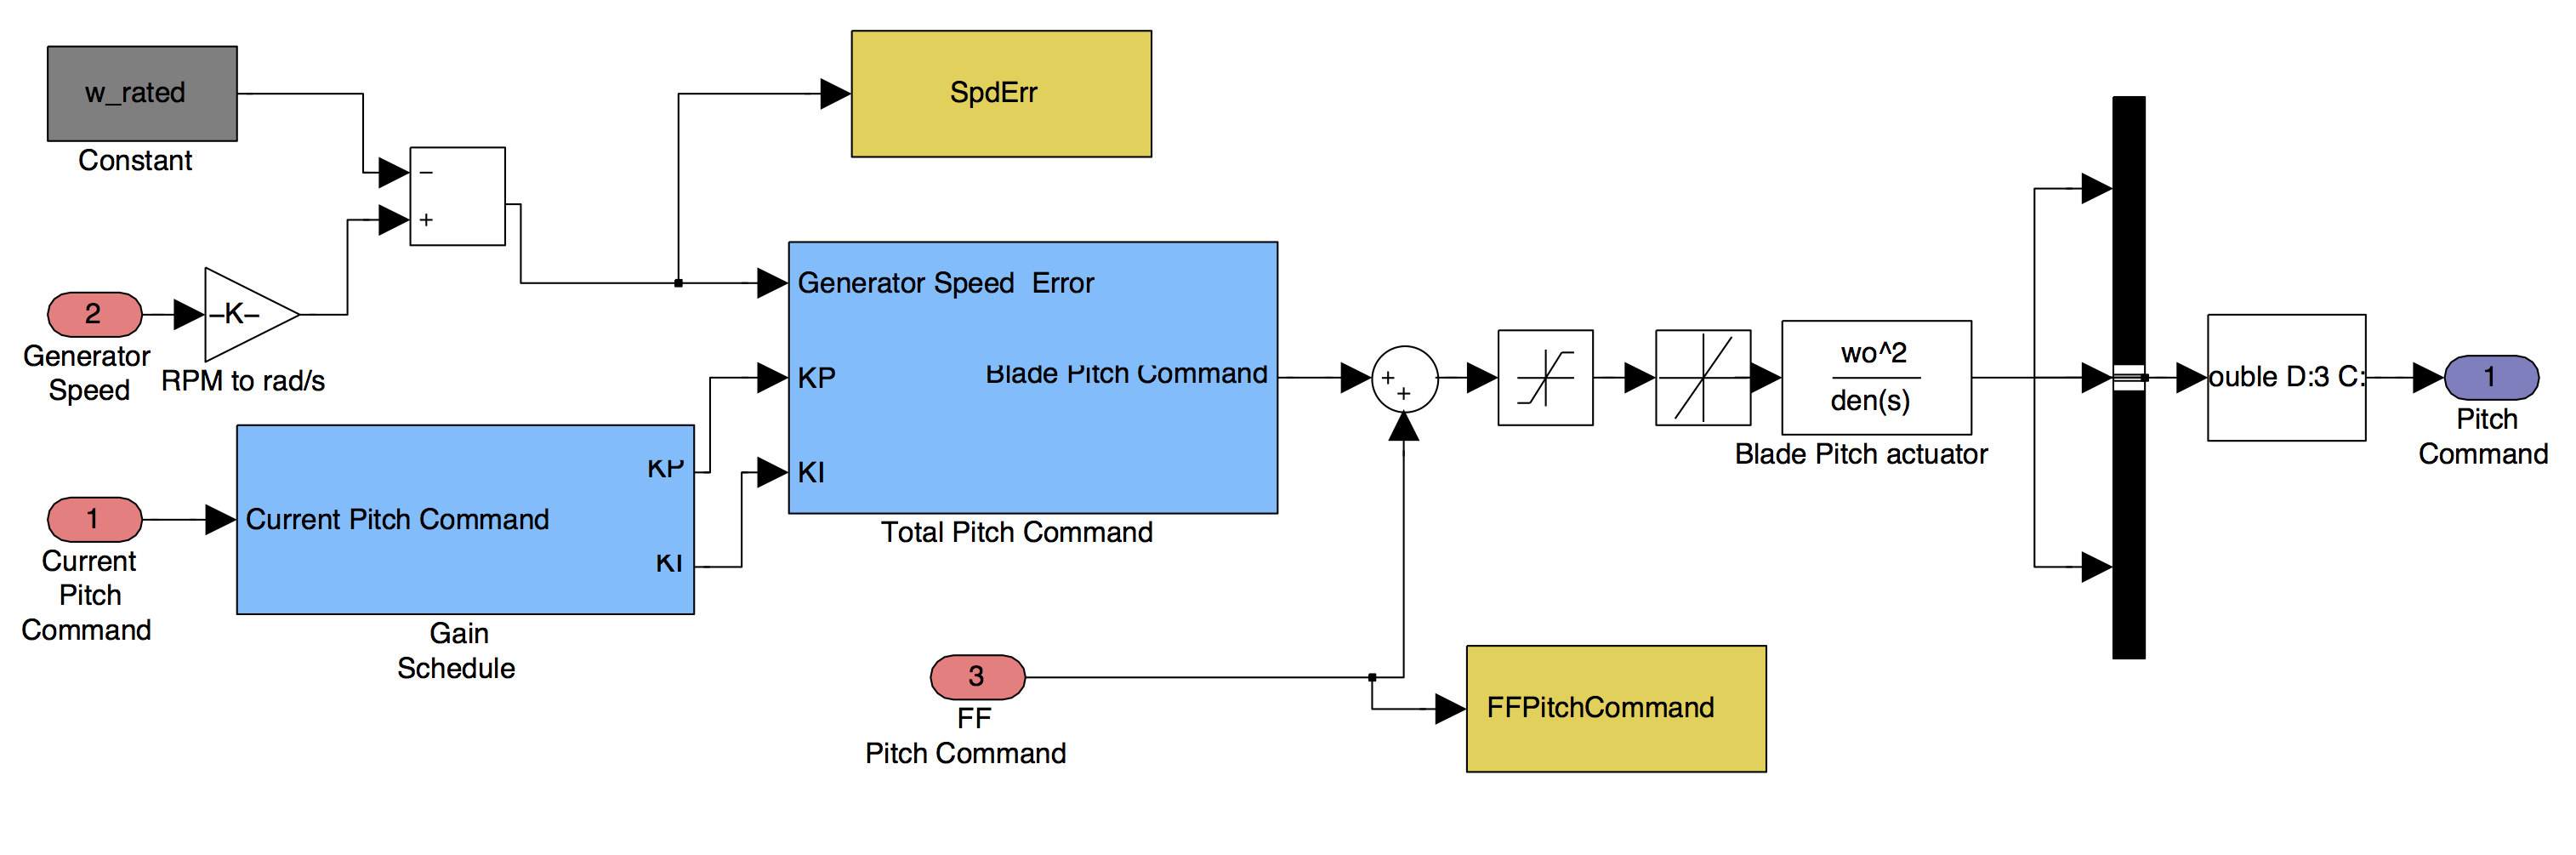
\includegraphics[width=\linewidth]{Figures/AppendixBFigures/FF_Pitch3.pdf}
	\caption{Pitch Controller subsystem for Simulink model of NREL 5-MW with feed forward optimal pitch control.}
	\label{figB-9}
\end{figure}

The Gain Schedule, Total Pitch Command, Torque Controller, and GenTorque subsystems are identical to the subsystems in the baseline NREL 5-MW controller, so they are not shown here. The form and function of those subsystems are described in Section \ref{sectionB-1}.

